\section{1174074 - Mochamad Arifqi Ramadhan}
\subsection{Soal Teori}
\begin{enumerate}
    \item Jelaskan dengan ilustrasi gambar sendiri apa itu generator dengan perumpamaan anda sebagai mahasiswa sebagai generatornya.
    \hfill\break
    Tugas Generator sekarang sedang dibuat untuk membuat koleksi gambar palsu, yang saat ini dilihat oleh Diskriminator. Diskriminator tidak dapat membedakan antara yang asli dan yang palsu. Untuk ilustrasi, lihat gambar berikut: 
    \begin{figure}[H]
		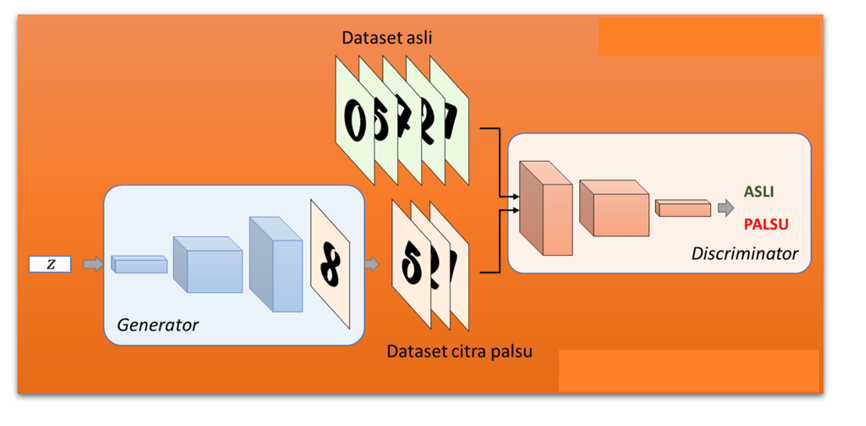
\includegraphics[width=4cm]{figures/1174074/8/teori1,2.png}
		\centering
		\caption{Teori 1}
    \end{figure}

    \item Jelaskan dengan ilustrasi gambar sendiri apa itu diskriminator dengan perumpamaan dosen anda sebagai diskriminatornya.
    \hfill\break
    Diskriminator adalah CNN yang menerima input gambar yang dimiliki dan menghasilkan angka biner yang meminta input gambar, lalu menghasilkan gambar dari dataset asli atau menghasilkan gambar palsu. Untuk ilustrasi, lihat gambar berikut: 
    \begin{figure}[H]
		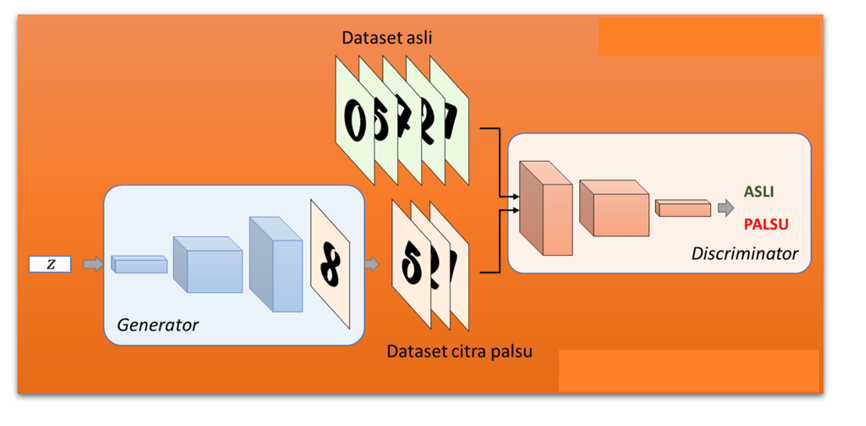
\includegraphics[width=4cm]{figures/1174074/8/teori1,2.png}
		\centering
		\caption{Teori 2}
    \end{figure}

    \item Jelaskan dengan ilustrasi gambar sendiri bagaimana arsitektur generator dibuat.
	\hfill\break
    Aksitektur generator dibuat bisa dijelaskan pada gambar berikut :
    \begin{figure}[H]
		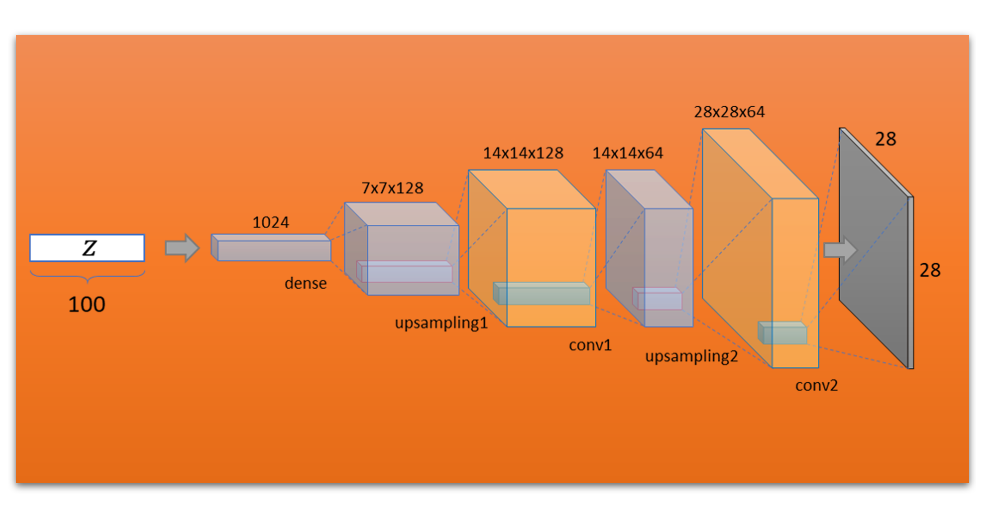
\includegraphics[width=4cm]{figures/1174074/8/teori3.png}
		\centering
		\caption{Teori 3}
    \end{figure}

    \item Jelaskan dengan ilustrasi gambar sendiri bagaimana arsitektur diskriminator dibuat.
	\hfill\break
    Aksitektur diskriminator dibuat bisa dijelaskan pada gambar berikut :
    \begin{figure}[H]
		\includegraphics[width=4cm]{figures/1174074/8/teori4.png}
		\centering
		\caption{Teori 4}
    \end{figure}

    \item Jelaskan dengan ilustrasi gambar apa itu latent space.
	\hfill\break
    Latent space dijelaskan pada gambar berikut :
    \begin{figure}[H]
		\includegraphics[width=4cm]{figures/1174074/8/teori5.png}
		\centering
		\caption{Teori 5}
    \end{figure}

    \item Jelaskan dengan ilustrasi gambar apa itu adversarial play.
	\hfill\break
    Adversarial play dijelaskan pada gambar berikut :
    \begin{figure}[H]
		\includegraphics[width=4cm]{figures/1174074/8/teori6.png}
		\centering
		\caption{Teori 6}
    \end{figure}

    \item Jelaskan dengan ilustrasi gambar apa itu Nash equilibrium.
	\hfill\break
	Nash equilibrium adalah Teori permainan adalah studi tentang interaksi strategis antara agen rasional. Sederhananya itu berarti itu adalah studi interaksi ketika pihak-pihak yang terlibat mencoba dan melakukan yang terbaik dari sudut pandang mereka, detailnya dapat dijelaskan pada gambar berikut : 
    \begin{figure}[H]
		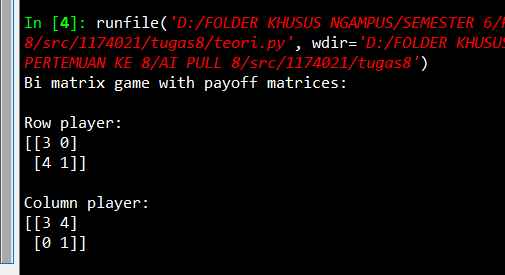
\includegraphics[width=4cm]{figures/1174074/8/teori7.png}
		\centering
		\caption{Teori 7}
    \end{figure}

    \item Sebutkan dan jelaskan contoh-contoh implementasi dari GAN.
	\hfill\break
	Menurut saya implementasi 3DGAN yaitu pada MAPS dan juga IKEA. Karena pada maps dan juga ikea sudah menerapkan bentuk 3 dimensi yang bisa lebih menarik perhatikan pengguna.

    \item Berikan contoh dengan penjelasan kode program beserta gambar arsitektur untuk membuat generator(neural network) dengan sebuah input layer, tiga hidden layer(dense layer), dan satu output layer(reshape layer).
	\hfill\break
    Untuk penjelasan tersebut dijelaskan pada gambar dibawah ini :
    \begin{figure}[H]
		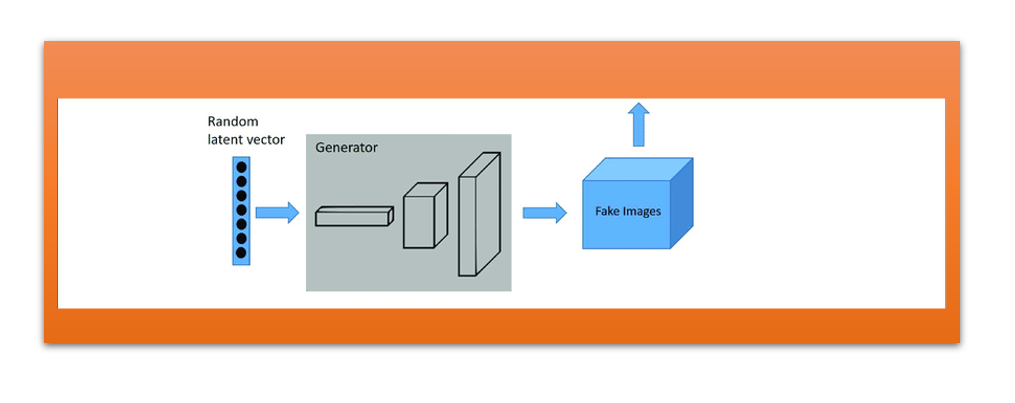
\includegraphics[width=4cm]{figures/1174074/8/teori9.png}
		\centering
		\caption{Teori 9}
    \end{figure}

    \item Berikan contoh dengan ilustrasi dari arsitektur dikriminator dengan sebuath input layer, 3 buah hidden layer, dan satu output layer.
	\hfill\break
    Untuk penjelasan tersebut dijelaskan pada gambar dibawah ini :
    \begin{figure}[H]
		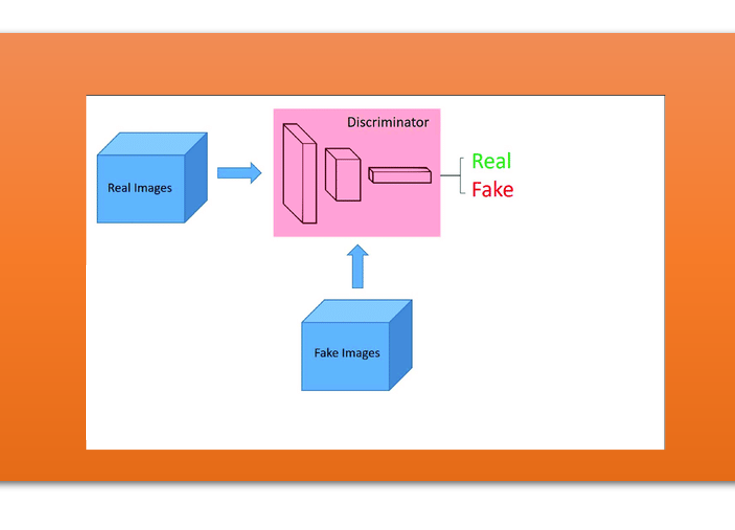
\includegraphics[width=4cm]{figures/1174074/8/teori10.png}
		\centering
		\caption{Teori 10}
    \end{figure}

    \item Jelaskan bagaimana kaitan output dan input antara generator dan diskriminator tersebut. Jelaskan kenapa inputan dan outputan seperti itu.
	\hfill\break
	Gambar dari Generator yang berhasil di deteksi oleh Diskriminator sebagai gambar fake, akan dikembalikan dengan feedback pke generator. Kini Generator bertugas untuk bisa membuat sekumpulan gambar palsu, yang nantinya dapat dilihat oleh Diskriminator, lalu, Diskriminator tidak bisa membedakan fake dan real.

	\item Jelaskan apa perbedaan antara Kullback-Leibler divergence (KL divergence)/relativeentropy, Jensen-Shannon(JS) divergence / information radius(iRaD) / total divergence to the average dalam mengukur kualitas dari model.
	\hfill\break
	Perbedaan nya yaitu memiliki model dari rumus yang berbeda-beda sehingga mempengaruhi hasil train dan test

	\item Jelaskan apa itu fungsi objektif yang berfungsi untuk mengukur kesamaan antara gambar yang dibuat dengan yang asli.
    \hfill\break
    Ukuran penting untuk menilai kualitas model. lalu kemudian akan melihat di keseimbangan Nash.

	\item Jelaskan apa itu scoring algoritma selain mean square error atau cross entropy seperti The Inception Score dan The Frechet Inception distance.
	\hfill\break
	The inception score adalah algoritma penilaian yang paling banyak digunakan untuk GAN. The Frechet Inception distance adalah Untuk mengatasi berbagai kekurangan Skor awal

	\item Jelaskan kelebihan dan kekurangan GAN.
	\hfill\break
	Kelebihan : GAN dapat memvisualiasikan bentuk model menjadi plot. Kemudian pada Kelemahan : model susah untuk implementasikan yang membuat data training menjadi lemah.
\end{enumerate}

\subsection{Praktek Program}
\begin{enumerate}
    \item Soal 1
    \hfill\break
    Konvolusi 3D. Konvolusi 3D menerapkan filter 3 dimensi ke kumpulan data dan filter 3 arah (x, y, z) untuk menghitung representasi fitur tingkat rendah. Bentuk outputnya adalah ruang volume 3 seperti kubus atau berbentuk kubus. 3D sangat membantu dalam pendeteksian peristiwa dalam video, gambar medis 3D, dll. Generative Adversarial Network adalah arsitektur jaringan saraf tiruan yang dimaksudkan untuk membuat atau membuat data yang benar-benar baru, dari nol hingga tidak ada sama sekali. Melihat target utama GAN adalah data gambar. Singkatnya, jaringan GAN berfungsi untuk memberikan gambar baru berdasarkan koleksi gambar yang telah ada sebelumnya selama proses training.

    \item Soal 2
	\hfill\break
	\lstinputlisting[firstline=34, lastline=64]{src/1174074/8/run.py}
	Kode di atas akan melakukan create generator ialah gloss, Bentuk jaringan Generator dapat dilihat berkebalikan dengan struktur jaringan saraf pada umumnya. Generator biasanya menerima input sebuah vektor z, yang kemudian mengubahnya menjadi sebuah output 3D atau 3 dimensi.

    \item Soal 3
	\hfill\break
	\lstinputlisting[firstline=69, lastline=107]{src/1174074/8/run.py}
	Diskrimanator adalah d\_loss, Jaringan Discriminator merupakan jaringan klasifikasi biner yang menerima input gambar tiga dimensi dan mengeluarkan klasifikasi menyatakan input gambar adalah gambar asli dari dataset atau merupakan gambar buatan Generator. Diskriminator dilatih dengan dataset yang diambil dari Generator, lalu di training untuk membedakan keduanya. Gambar dari Generator yang berhasil di deteksi oleh Diskriminator sebagai gambar fake, akan dikembalikan dengan feedback pke generator. Kini Generator bertugas untuk bisa membuat sekumpulan gambar palsu, yang nantinya dapat dilihat oleh Diskriminator, lalu, Diskriminator tidak bisa membedakan fake dan real.

    \item Soal 4
	\hfill\break
    Proses training 3D GAN yaitu dengan melakukan epoch sebanyak yang ditentukan.
    
    \item Soal 5
	\hfill\break
	\begin{itemize}
		\item Clone github
		\item Download dataset
		\item Buat folder baru logs dan results
	\end{itemize}

	\item Soal 6
	\hfill\break
	Dataset yang digunakan yaitu 3DShapeNets yang berisi model model bentuk benda dll, folder train berisi train dan folder test berisi data testing. dan semua data tersebut di simpan didalam folder volumetric\_data.

    \item Soal 7
	\hfill\break
	Volume pixel atau voxel adalah titik dalam ruang tiga dimensi. Sebuah voxel mendefinisikan posisi dengan tiga koordinat dalam arah x, y, dan z. Sebuah voxel adalah unit dasar untuk mewakili gambar 3D. Untuk gambar nya ialah sebagai berikut :
    \begin{figure}[H]
		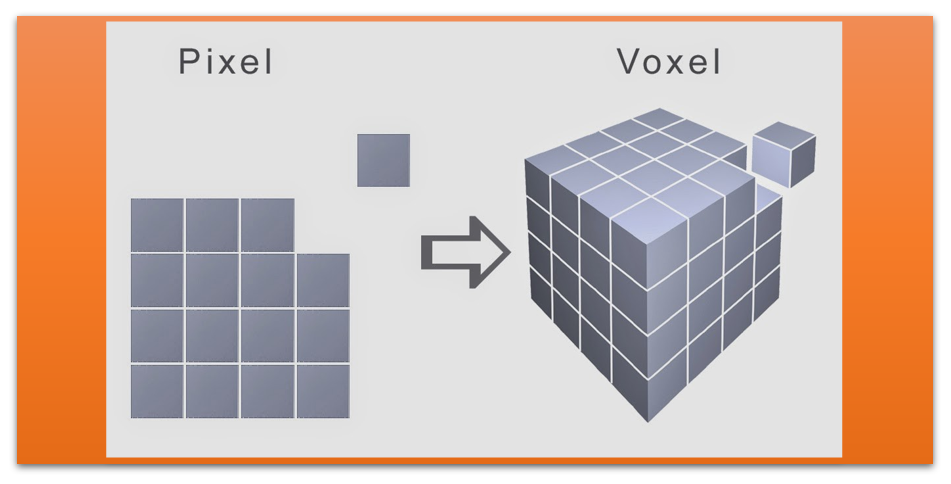
\includegraphics[width=4cm]{figures/1174074/8/praktek7.png}
		\centering
		\caption{Praktek 7}
    \end{figure}

    \item Soal 8
	\hfill\break
	\lstinputlisting[firstline=1, lastline=28]{src/1174074/8/display.py}
	Kode di atas befungsi untuk visualisasidataset dalam tampilan plot. langkah-langkah seperti ini :
    import library, load data file .mat dan lakukan read memakai matplotlib, Hasilnya adalah sebagai berikut :
    \begin{figure}[H]
		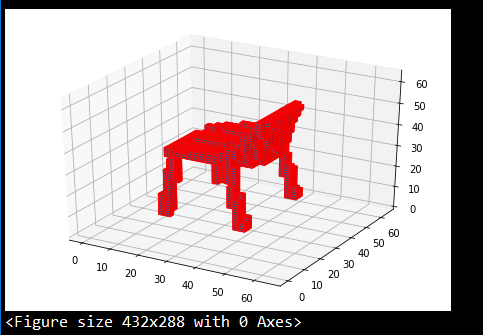
\includegraphics[width=4cm]{figures/1174074/8/praktek8.png}
		\centering
		\caption{Praktek 8}
    \end{figure}

    \item Soal 9
	\hfill\break
	\lstinputlisting[firstline=32, lastline=64]{src/1174074/8/run.py}
	Kode di atas befungsi untuk membuat generator yaitu dengan ketentukan gen sebagai variabel dan membuat fungsi atau variabel genmodel lalu dilakukan return. 

    \item Soal 10
	\hfill\break
	\lstinputlisting[firstline=66, lastline=107]{src/1174074/8/run.py}
	Kode di atas befungsi untuk membangun diskriminator berfungsi untuk mendefenisikan seluruh gambar yang sudah di load generator sebagai gambar fake dan real.

    \item Soal 11
	\hfill\break
	Jika interpreter python menjalankan if name == main sebagai program utama, itu ialah menetapkan variabel name untuk memiliki nilai main. Jika file ini sedang di impor dari modul lain, name akan ditetapkan ke nama modul. Nama modul tersedia sebagai nilai untuk name variabel global.

    \item Soal 12
	\hfill\break
	\lstinputlisting[firstline=164, lastline=174]{src/1174074/8/run.py}
	Kode di atas befungsi untuk melakukan load dataset dengan ketentuan data yang hanya dalam folder chair pada data train.

    \item Soal 13
	\hfill\break
	\lstinputlisting[firstline=176, lastline=187]{src/1174074/8/run.py}
    Kode di atas menggunakan Adam sebagai algoritma pengoptimalan dan binary\_crossentropy sebagai kerugian loss. 
    
    \item Soal 14
	\hfill\break
	\lstinputlisting[firstline=189, lastline=196]{src/1174074/8/run.py}
	Kode di atas artinya ialah kita memasukkan random vector kedalam generator model lalu membagi 2 yaitu generated example dan real example, dan meneruskan ke diskriminator model sebagai real atau fake

    \item Soal 15
	\hfill\break
	\lstinputlisting[firstline=198, lastline=202]{src/1174074/8/run.py}
    Kode di atas befungsi untuk melakukan load data pada dataset.
    
    \item Soal 16
	\hfill\break
	\lstinputlisting[firstline=204, lastline=207]{src/1174074/8/run.py}
    Kode di atas berfungsi untuk membuat tensorboard yang nantinya bisa diakses melalui localhost.
    
    \item Soal 17
	\hfill\break
	\lstinputlisting[firstline=209, lastline=211]{src/1174074/8/run.py}
    Kode di atas befungsi untuk melakukan reshape agar shape yang dihasilkan tidak terlalu besar. Dengan membuat variabel real dan fake.
    
    \item Soal 18
	\hfill\break
	\lstinputlisting[firstline=213, lastline=219]{src/1174074/8/run.py}
	Kode di atas befungsi untuk melakukan training epoch, karena jika epoch semakin banyak maka kualiatas training yang dihasilkan akan semakin baik.

    \item Soal 19
	\hfill\break
	\lstinputlisting[firstline=221, lastline=225]{src/1174074/8/run.py}
    Batch adalah jumlah file yang akan di training.
    
    \item Soal 20
	\hfill\break
	\lstinputlisting[firstline=274, lastline=229]{src/1174074/8/run.py}
    Kode di atas befungsi untuk untuk membuat gambar bersih dari noise dan juga menyesuaikan shape.
    
    \item Soal 21
	\hfill\break
	\lstinputlisting[firstline=231, lastline=233]{src/1174074/8/run.py}
    Kode di atas befungsi untuk membuat sample gambar palsu yang akan diteruskan ke diskriminator.
    
    \item Soal 22
	\hfill\break
	\lstinputlisting[firstline=239, lastline=249]{src/1174074/8/run.py}
	Kode di atas befungsi untuk membuat diskriminator bisa load gambar fake dan real dari generator, oleh karena itu ada generator loss dan diskriminator loss untuk melihat seberapa baik kualitas yang dihasilkan.

    \item Soal 23
	\hfill\break
	\lstinputlisting[firstline=251, lastline=261]{src/1174074/8/run.py}
    Kode di atas befungsi untuk melakukan print gloss untuk generator dan juga dloss untuk diskriminator.
    
    \item Soal 24
	\hfill\break
	\lstinputlisting[firstline=263, lastline=742]{src/1174074/8/run.py}
    Mengapa ada perulangan ? karena untuk melakukan perbandingan dari hasil yang sudah didapat.
    
    \item Soal 25
	\hfill\break
	\lstinputlisting[firstline=744, lastline=747]{src/1174074/8/run.py}
    TensorBoard adalah sebuah aplikasi web localhost untuk memeriksa dan menyelesaikan grafik dari hasil TensorFlow.
    
    \item Soal 26
	\hfill\break
	\lstinputlisting[firstline=283, lastline=285]{src/1174074/8/run.py}
    File H5 adalah file data yang disimpan dalam Format Data Hirarki (HDF). Ini berisi array multidimensi data ilmiah.
    
    \item Soal 74
	\hfill\break
	\lstinputlisting[firstline=287, lastline=305]{src/1174074/8/run.py}
    Ini adalah tahap akhir untuk melakukan testing dari model yang telah dibuat dan buat model dari yang sudah di create sebelumnya yaitu generator dan diskriminator. Untuk ilustrasi gambar sebagai berikut : 
    \begin{figure}[H]
		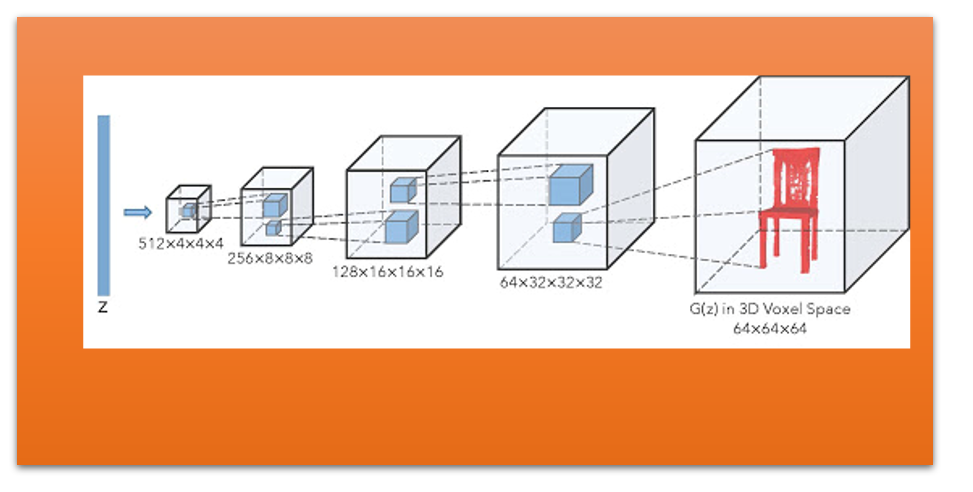
\includegraphics[width=4cm]{figures/1174074/8/praktek74.png}
		\centering
		\caption{Praktek 74}
    \end{figure}
\end{enumerate}
\subsection{Penanganan Error}

\subsection{Bukti Tidak Plagiat}
\begin{figure}[H]
    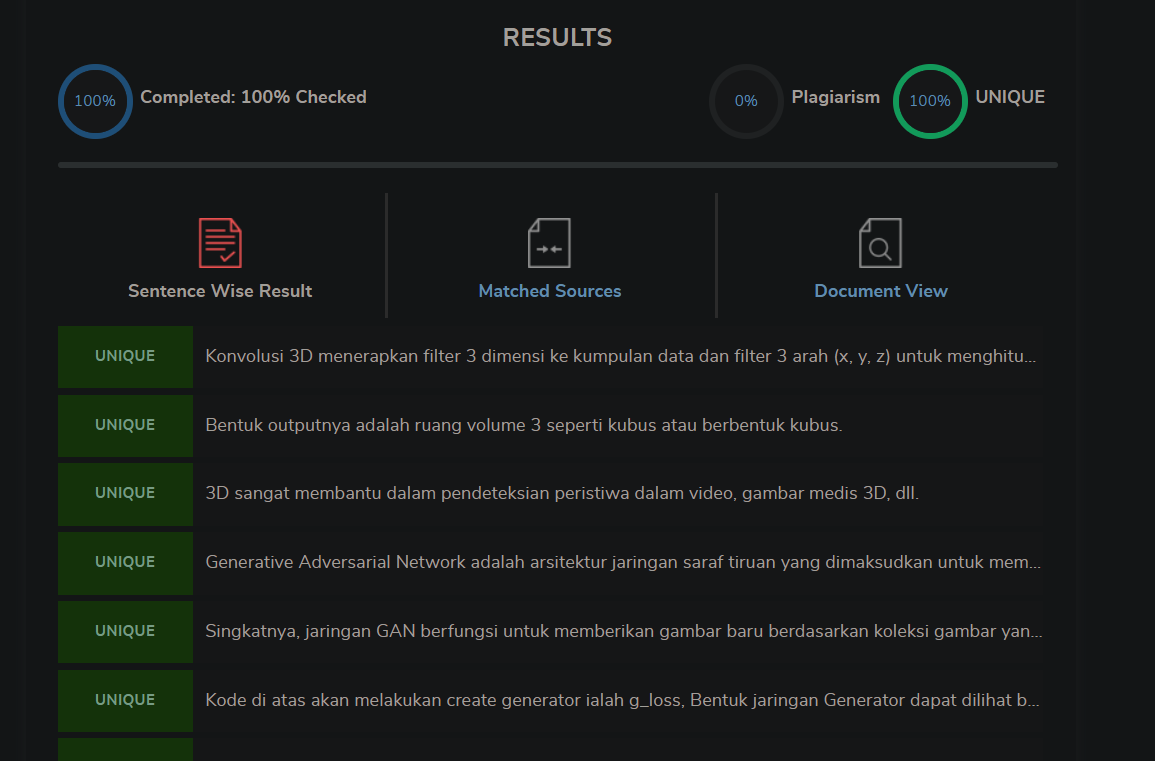
\includegraphics[width=4cm]{figures/1174074/8/8.png}
    \centering
    \caption{Bukti Tidak Melakukan Plagiat Chapter 8}
\end{figure}